\begin{figure}[!ht]
    \centering
    \setlength{\resLen}{1.4in}
    \addtolength{\tabcolsep}{-3.5pt}
    \begin{tabular}{cccc}
        \multicolumn{4}{c}{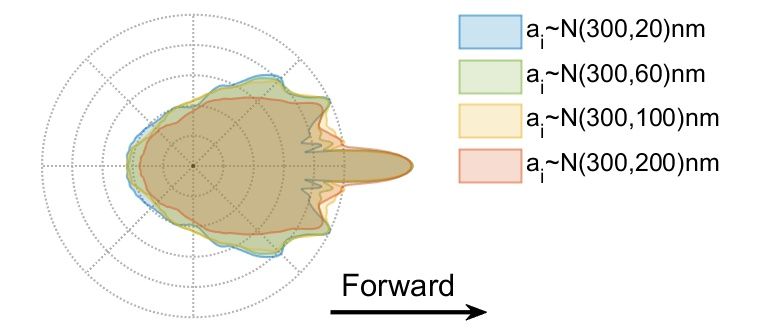
\includegraphics[width=3.\resLen]{waveoptics/pfunc/radius_gaussian.jpg}} \\ [-1em]
        \includegraphics[width=\resLen]{waveoptics/particle/sigma_0.02.jpg} &
        \includegraphics[width=\resLen]{waveoptics/particle/sigma_0.06.jpg} &
        \includegraphics[width=\resLen]{waveoptics/particle/sigma_0.1.jpg} &
        \includegraphics[width=\resLen]{waveoptics/particle/sigma_0.2.jpg} 
        \\ [-1em]
        \includegraphics[width=\resLen]{waveoptics/lucy/sigma_0.02.jpg} &
        \includegraphics[width=\resLen]{waveoptics/lucy/sigma_0.06.jpg} &
        \includegraphics[width=\resLen]{waveoptics/lucy/sigma_0.1.jpg} &
        \includegraphics[width=\resLen]{waveoptics/lucy/sigma_0.2.jpg} \\
        $\mathcal{N}(300,20)\,$nm & $\mathcal{N}(300,60)\,$nm & $\mathcal{N}(300,100)\,$nm & $\mathcal{N}(300,200)\,$nm
    \end{tabular}
    \caption[Comparison with different radius distribution]{\label{fig:waveoptics:paritclesize}
        Comparison of the resulting phase function and rendering for different particle radius distribution. They have the same mean radius but different variations.
    }
\end{figure}

